\documentclass[../notes.tex]{subfiles}

\pagestyle{main}
\renewcommand{\chaptermark}[1]{\markboth{\chaptername\ \thechapter\ (#1)}{}}
\setcounter{chapter}{5}

\begin{document}




\chapter{Magnetochemistry}
\section{Magnetochemistry I}
\begin{itemize}
    \item \marginnote{2/7:}Extension from last time: Deriving the relationship between two simple harmonic oscillators' fundamental frequencies and reduced masses.
    \begin{itemize}
        \item Suppose you have two homonuclear diatomic molecules \ce{A-A} and \ce{B-B}, and you wish to relate their vibrational frequencies.
        \item Reduced masses of the molecules.
        \begin{align*}
            \mu_{\ce{AA}} &= \frac{m_{\ce{A}}m_{\ce{A}}}{m_{\ce{A}}+m_{\ce{A}}}&
            \mu_{\ce{BB}} &= \frac{m_{\ce{B}}m_{\ce{B}}}{m_{\ce{B}}+m_{\ce{B}}}
        \end{align*}
        \item Vibrational frequencies of the molecules in terms of the reduced masses.
        \begin{align*}
            \nu_{\ce{AA}} &= k\sqrt{\frac{F}{\mu_{\ce{AA}}}}&
            \nu_{\ce{BB}} &= k\sqrt{\frac{F}{\mu_{\ce{BB}}}}
        \end{align*}
        \item Take the ratio of the above two quantities to relate them.
        \begin{equation*}
            \frac{\nu_{\ce{AA}}}{\nu_{\ce{BB}}} = \frac{k\sqrt{\frac{F}{\mu_{\ce{AA}}}}}{k\sqrt{\frac{F}{\mu_{\ce{BB}}}}}
            = \frac{\sqrt{\mu_{\ce{BB}}}}{\sqrt{\mu_{\ce{AA}}}}
        \end{equation*}
    \end{itemize}
    \item Today: Magnetochemistry.
    \begin{itemize}
        \item 1-2 lectures on this.
        \item \textcite{bib:CHEM20100Notes} has a good write-up of the derivation at the beginning of today's lecture.
        \begin{itemize}
            \item See Module 34: Magnetic Properties of Transition Metal Complexes.
        \end{itemize}
        \item \textcite{bib:CHEM20200Notes} has more on the content at the end of the lecture.
        \begin{itemize}
            \item See Lecture 3: TM Magnetism.
        \end{itemize}
    \end{itemize}
    \item Magnetism really is the province of inorganic chemistry since it's here that we find the compounds with unpaired electrons.
    \begin{itemize}
        \item Organic compounds don't have these outside of free radicals.
    \end{itemize}
    \item We begin with some terminology and relations.
    \item \textbf{Magnetic field}. \emph{Denoted by} $\bm{H}$, $\bm{\vec{H}}$.
    \begin{itemize}
        \item $H$ denotes the magnitude of $\vec{H}$.
    \end{itemize}
    \item \textbf{Magnetization}: The response of the electrons in a material to a magnetic field. \emph{Denoted by} $\bm{M}$.
    \begin{itemize}
        \item Alternatively: The magnetic moment per unit volume.
        \item Everything with electrons has \emph{some} degree of a response to a magnetic field.
        \item Depends on the strength of the field in which the material is placed.
    \end{itemize}
    \item \textbf{Magnetic induction}: The density of magnetic field lines within a substance. \emph{Denoted by} $\bm{B}$. \emph{Units} Teslas or Gauss.
    \begin{itemize}
        \item $\SI{1}{\tesla}=\SI{10000}{\gauss}$.
        \item The scale of these units.
        \begin{itemize}
            \item The Earth's magnetic field is about \SI{3.1e-5}{\tesla}.
            \item A \SI{900}{\mega\hertz} NMR spectrometer is about \SI{21}{\tesla}.
            \item An MRI is about \SIrange{1.3}{3}{\tesla}.
        \end{itemize}
    \end{itemize}
    \item We now give a few relations between the above quantities.
    \item First, we have that
    \begin{equation*}
        B = \frac{F}{Qv}
    \end{equation*}
    where $F$ is in Newtons, $Q$ is in Coulombs, and $v$ is in meters per second.
    \item Additionally, placing a sample with magnetization $M$ in a magnetic field $\vec{H}$ alters the magnetic induction via
    \begin{equation*}
        B = \vec{H}+4\pi\vec{M}
    \end{equation*}
    \item Magnetically isotropic substances in a uniform magnetic field experience no force.
    \item In a region of nonhomogeneous field strength, a force is exerted along the axis of the field gradient as described by
    \begin{equation*}
        \vec{f} = \vec{M}\cdot\dv{H}{z}
    \end{equation*}
    \item \textbf{Magnetic susceptibility}. \emph{Denoted by} $\bm{\chi}$.
    \begin{itemize}
        \item A tensor of rank 2.
        \item We have that $\vec{M}=\vec{\chi}\vec{H}$.
    \end{itemize}
    \item There are different types of $\chi$.
    \item \textbf{Volume susceptibility}: \emph{Denoted by} $\bm{\chi_V}$. \emph{Units} \si{\electromagneticunit\per\cubic\centi\meter}. \emph{Given by}
    \begin{equation*}
        \chi_V = \chi = \frac{\vec{M}}{\vec{H}}
    \end{equation*}
    \begin{itemize}
        \item This is a dimensionless quantity, but we still use the units listed above.
        \item Note that an emu is an "electromagnetic unit."
    \end{itemize}
    \item \textbf{Gram susceptibility}: \emph{Denoted by} $\bm{\chi_g}$. \emph{Units} \si{\cubic\centi\meter\per\gram}. \emph{Given by}
    \begin{equation*}
        \chi_g = \frac{\chi_V}{d}
    \end{equation*}
    \item \textbf{Molar susceptibility}: \emph{Denoted by} $\bm{\chi_M}$. \emph{Units} \si{\cubic\centi\meter\per\mole}. \emph{Given by}
    \begin{equation*}
        \chi_m = \chi_g\cdot\text{MW}
    \end{equation*}
    \item The sign of $\chi$ ($+/-$) depends on the presence or absence of unpaired electrons. In particular\dots
    \begin{itemize}
        \item $\chi>0$ indicates unpaired electrons.
        \item $\chi<0$ indicates paired electrons.
    \end{itemize}
    \item We now move on to diamagnetism.
    \item Most matter is diamagnetic.
    \item \textbf{Diamagnetic} (compound): A compound that has no unpaired electrons. \emph{Also known as} \textbf{diamagnet}.
    \begin{itemize}
        \item $S=0$ for a diamagnet.
        \item These materials are weakly repelled by magnetic fields.
        \item The old-school way to measure this weak repulsion is with a \textbf{Gouy balance}.
    \end{itemize}
    \item \textbf{Gouy balance}: An instrument that measures the change in mass of a sample as it is attracted ore repelled by a powerful magnetic field.
    \begin{figure}[h!]
        \centering
        \begin{tikzpicture}
            \footnotesize
            \draw (-1.5,0) -- ++(1,0) -- node[left]{$N$} ++(0,0.5) -- ++(-1,0);
            \draw (1.5,0) -- ++(-1,0) -- node[right]{$S$} ++(0,0.5) -- ++(1,0);
            \draw [dashed] (-0.5,0.25) -- ++(1,0);
    
            \draw [semithick,-latex] (0,0.8) -- ++(0,-1);
            \fill [blz] (-0.1,1) -- (-0.1,0.8) to[out=-90,in=-90,looseness=2] (0.1,0.8) -- (0.1,1) -- cycle;
            \draw [gray,thick] (-0.1,1.5) -- (-0.1,0.8) to[out=-90,in=-90,looseness=2] (0.1,0.8) -- (0.1,1.5) -- cycle;
            \draw (0,1.5) -- ++(0,0.5) -- ++(1,0) -- ++(0,-0.3) node[below]{scale};
        \end{tikzpicture}
        \caption{Gouy balance.}
        \label{fig:Gouy}
    \end{figure}
    \begin{itemize}
        \item Historically, varying a magnetic field precisely has been very difficult (we didn't always have electromagnets into which we could just dial any field).
        \begin{itemize}
            \item In fact, even today, varying a magnetic field super precisely is difficult. This is why NMR machines vary the frequency domain over a constant magnetic field (as opposed to varying the magnetic domain over a constant frequency).
        \end{itemize}
        \item Under a constant magnetic field, the sample (contained in an NMR tube) is linked to a scale. As the sample moves through that field, it experiences a changing magnetic field.
        \item The change in mass of the sample at different points in the field gives information on its magnetic susceptibility.
    \end{itemize}
    \item Modern update to the Gouy balance: The superconducting quantum interference device, or SQUID.
    \begin{itemize}
        \item We still measure the magnetic susceptibility essentially the same way, just with fancier toys.
        \item Today, we move our sample through an electromagnet-generated magnetic field and then see what kind of current gets induced in a superconducting coil (recall that moving magnets induce currents).
        \item The underlying physics is well beyond the scope of this course, but also fascinating. It involves \textbf{Josephson junctions}, etc.
    \end{itemize}
    \item \textbf{Diamagnetic magnetic susceptibility}. \emph{Denoted by} $\bm{\chi_\textbf{dia}}$.
    \item Since all electrons are \emph{paired} in a diamagnetic compound, we have by the above that $\chi_\text{dia}<0$.
    \item Diamagnetic contributions can be calculated as follows.
    \begin{equation*}
        \chi_\text{dia} = \sum\lambda+\sum n_i\chi_i
    \end{equation*}
    \begin{itemize}
        \item $\lambda$ is a \textbf{constitutive correction} related to ring currents for bonds/ring delocalization.
        \item $n_i\chi_i$ is contributions from individual atoms.
    \end{itemize}
    \item The values in the above equation can be looked up for a compound.
    \begin{itemize}
        \item In particular, see \textcite{bib:BerryDiamagnetism}.
        \item The paper has a nice introduction and does the derivation that Anderson just did, too.
        \item Then it contains a bunch of tables of different corrections for various bond types.
        \item These values are all pretty small, so it doesn't really matter if you just miss one or two things in ambiguous cases, but Anderson tries to sum over all of them.
        \item You \emph{do} need to do these corrections when you're doing a lot of these calculations.
        \begin{itemize}
            \item The result will be on the order of \SI{e-6}{\electromagneticunit}, but that can be significant enough to effect your work.
        \end{itemize}
        \item These tables give both $\lambda$ and $\chi_i$ values; you need to sum over the individual atom $\chi_i$ values and then constitutive corrections for groups. For example, for a \ce{Cp} group, you have 5 carbons, 5 hydrogens, and a constitutive correction for the whole group (which should be equal to that of 5 carbons, 5 hydrogens, and 5 \ce{C=C} double bonds??).
        \item These values are field-independent and pretty constant.
    \end{itemize}
    \item That's the contribution from paired electrons. What we really care about in general are the unpaired electrons, though.
    \item Paramagnetism.
    \item \textbf{Paramagnetic} (compound): A compound that has unpaired electrons. \emph{Also known as} \textbf{paramagnet}.
    \begin{itemize}
        \item Positive $\chi$ values; thus, they get pulled into applied magnetic fields.
    \end{itemize}
    \item Temperature dependence of $\chi$.
    \begin{itemize}
        \item There is an inversely proportional relationship between $\chi$ and $T$; in other words, a plot of $1/\chi$ vs. $T$ is linear.
        \item This notion is formalized by \textbf{Curie's law}.
    \end{itemize}
    \item \textbf{Curie constant}: The following constant. \emph{Denoted by} $\bm{C}$. \emph{Given by}
    \begin{equation*}
        C = \frac{\NA g^2\mB^2(S(S+1))}{3\kB}
    \end{equation*}
    \begin{itemize}
        \item $g$ is the \textbf{gyromagnetic ratio}.
        \item $\mB$ is the Bohr magneton.
        \item $\NA$ is Avogadro's number.
        \item $S$ is the spin quantum number.
    \end{itemize}
    \item \textbf{Gyromagnetic ratio}: The quotient of the magnetic moment of an electron by its angular momentum. \emph{Also known as} \textbf{magnetogyric ratio}. \emph{Denoted by} $\bm{g}$.
    \begin{itemize}
        \item There are even more names that the gyromagnetic ratio is sometimes called, just for added complexity :)
        \item Any fundamental particle can have one of these.
        \item Nuclei have them, but we're only worried about electrons here.
        \item Magnetic moment divided by angular momentum.
        \item 2.011 for electrons.
        \item More on this later.
    \end{itemize}
    \item \textbf{Curie's law}: The relationship between $\chi$ and $T$. \emph{Given by}
    \begin{equation*}
        \chi = \frac{C}{T}
    \end{equation*}
    \item From the written notes: We have that
    \begin{equation*}
        \mB = \frac{e\hbar}{2m_e} = \SI{9.3e-24}{\joule\per\tesla}
    \end{equation*}
    \item We want to take the picture provided by Curie's law and simplify it down now.
    \item For the spin-only case (this restriction is very important), we can define the effective magnetic moment
    \begin{equation*}
        \mu_\text{eff} = \sqrt{\frac{3\kB}{\NA\mB^2}}\sqrt{\chi T}
        = 2.828\sqrt{\chi T}
        = \sqrt{g^2(S(S+1))}
    \end{equation*}
    \begin{itemize}
        \item What is the origin of the first equality??
    \end{itemize}
    \item We also frequently write
    \begin{equation*}
        \chi T = \frac{\NA g^2\mB^2}{3\kB}(S(S+1))
        = \frac{g^2}{8}(S(S+1))
    \end{equation*}
    \item Magnetochemists almost exclusively use $\chi T$, but $\mu_\text{eff}$ is oft reported for room temp characterizations.
    \item Know the end results below: Very important for how stuff is computed and talked about in the lit.
    \begin{align*}
        \mu_\text{eff} &= \sqrt{g^2(S(S+1))}&
        \chi T &= \frac{g^2}{8}S(S+1)
    \end{align*}
    \begin{itemize}
        \item Approximating $g\approx 2$, we can rewrite the above as
        \begin{align*}
            \mu_\text{eff} &= \sqrt{4(S(S+1))}&
            \chi T &= \frac{1}{2}S(S+1)
        \end{align*}
        \item $g\not\approx 2$ always, though --- take a look at the following examples.
    \end{itemize}
    \item Elements and some paramagnetic parameters.
    \begin{table}[h!]
        \centering
        \small
        \renewcommand{\arraystretch}{1.2}
        \begin{tabular}{c|cccc}
             & $S$ & $\mu_\text{eff}$ & $\chi T_\text{SO}$ & $\mu_\text{exp}$\\
            \hline
            \ce{Cu^2+} & 1/2 & 1.73 & 0.375 & \numrange{1.7}{2.2}\\
            \ce{Ni^2+} & 1 & 2.83 & 1 & \numrange{2.8}{3.5}\\
            \ce{Cr^3+} & 3/2 & 3.87 & 1.875 & \numrange{3.7}{3.9}\\
            \ce{Fe^2+} HS & 2 & 4.90 & 3 & \numrange{5.1}{5.7}\\
            \ce{Fe^3+} HS & 5/2 & 5.92 & 4.375 & \numrange{5.7}{6}\\
        \end{tabular}
        \caption{Magnetic parameters for example elements.}
        \label{tab:exampleElementsMagnetism}
    \end{table}
    \begin{itemize}
        \item Notation: SO for spin only. HS for high spin. exp for experimental.
        \item To calculate the data in Table \ref{tab:exampleElementsMagnetism}, find the number of unpaired electrons and go from there.
        \item Example: \ce{Cu^2+}. From the periodic table, \ce{Cu^2+} is $d^9$. Hence it has 1 unpaired electron. Thus\dots
        \begin{itemize}
            \item $S=1\cdot 1/2=1/2$.
            \item $\mu_\text{eff}=\sqrt{4(S(S+1))}=\sqrt{4(1/2(1/2+1))}=\sqrt{3}=1.73$.
            \item $\chi T_\text{SO}=1/2\cdot S(S+1)=1/2\cdot 1/2(1/2+1)=3/8=0.375$.
            \item The calculated effective $\mu$ often (not always) agrees with the experimental range.
        \end{itemize}
    \end{itemize}
    \item We now move on to spin-orbit coupling.
    \item Spin-orbit coupling: $g>0$ for a more-than-half-filled shell; $g<0$ for a less-than-half-filled shell.
    \item Consider a generic metal \ce{M} with $S=1/2$ and another with $S=1/2$ and a bridging ligand \ce{L} between them.
    \begin{itemize}
        \item Three possibilities to determine magnetism: The spins can be coupled antiferromagnetically (opposite directions) so $S=0$, coupled ferromagnetically so $S=1$, or uncoupled so both behave as their own spin center but are chemically/mechanically linked within the molecule.
    \end{itemize}
    \item Now for a specific example of metal centers with different spins: Consider \ce{Cu-L-Mn}, which has $S=1/2$ and $S=5/2$. Then
    \begin{equation*}
        \prb{\mu} = \sqrt{\mu_{\ce{Cu}}^2+\mu_{\ce{Mn}}^2}
        = \sqrt{3+35}
        = 6.16\mB
    \end{equation*}
    \begin{itemize}
        \item How does this work?? What is $\prb{\mu}$?
        \item Alternatively, $\chi T$ can be calculated (this is easier??).
    \end{itemize}
    \item A brief note about temperature-independent paramagnetism.
    \begin{itemize}
        \item If we measure \ce{Cu^{II}} and \ce{Co^{II}}, we get \SI{60e-6}{emu} and \SI{400e-6}{emu}.
        \begin{itemize}
            \item These come from excited state mixing: These excited states are not thermally populated, but they are a quantum mechanically admixed state (what does this mean??).
            \item What are these values??
        \end{itemize}
    \end{itemize}
    \item Note: Curie's law doesn't always hold. In cases where it doesn't, we can correct it to the \textbf{Curie-Weiss law}.
    \item \textbf{Weiss constant}: A constant describing certain magnetic interactions. \emph{Denoted by} $\bm{\theta}$.
    \begin{itemize}
        \item $\theta=0$ for a pure paramagnet.
        \item $\theta\neq 0$ for a long range magnetic interaction in a solid sample.
    \end{itemize}
    \item \textbf{Curie-Weiss law}: The following relation, where $C$ is the Curie constant, $T$ is temperature, and $\theta$ is the Weiss constant. \emph{Given by}
    \begin{equation*}
        \chi = \frac{C}{T-\theta}
    \end{equation*}
    \begin{itemize}
        \item Don't rush to use the Curie-Weiss law if your data isn't fitting to Curie's law, though: Magnetic measurements are very sensitive and 90\% of the time you're data isn't fitting, it's because your sample isn't clean.
    \end{itemize}
    \item We now return to the question of when $g$ deviates from 2: Indeed, this only happens when there is a substantial magnetic contribution from the orbital angular momentum.
    \item $S$ is our spin angular momentum quantum number, and $L$ is our orbital angular momentum quantum number.
    \begin{itemize}
        \item If spin and orbital angular momenta couple, then $S,L$ are no longer good quantum numbers.
        \item To fix this problem, we define a new one: $J$.
    \end{itemize}
    \item We define $J=L+S$ to characterize coupling.
    \begin{itemize}
        \item $J$ is very important with the lanthanides where our coupling is extremely large.
        \begin{itemize}
            \item In fact, in the lanthanides, coupling is so strong that you have to start with only a $J$ quantum number.
            \item For first-row transition metals, we treat $J$ just as a perturbation.
        \end{itemize}
    \end{itemize}
    \item We know that
    \begin{align*}
        L &= \sum_i\ell_i&
        S &= \sum_is_i
    \end{align*}
    \item Thus, our Hamiltonian is
    \begin{equation*}
        H = \hat{H}_0+\hat{H}_\text{elec}+\hat{H}_\text{SO}
    \end{equation*}
    \begin{itemize}
        \item SO denotes spin-orbit.
        \item We have that
        \begin{equation*}
            \hat{H}_\text{SO} = \lambda\hat{L}\cdot\hat{S}+\beta(\hat{L}+g_e\hat{S})-H
        \end{equation*}
        where $\lambda$ is the SOC constant.
        \item The energy that we get out of this Hamiltonian is
        \begin{equation*}
            E_n = E_n^0+HE_n^1+H^2E_n^2
        \end{equation*}
        \begin{itemize}
            \item The first-order correction is \textbf{Zeeman}; the second-order is \textbf{2nd order Zeeman}.
        \end{itemize}
    \end{itemize}
    \item An intuitive mental picture of SOC.
    \begin{itemize}
        \item Consider a perfectly octahedral $d^1$ complex.
        \item The electron can migrate through a degenerate set of orbitals, inducing a ring current.
        \item This is a useful classical analogy with predictive power.
        \begin{itemize}
            \item However, it is not quantum mechanically accurate at all.
        \end{itemize}
    \end{itemize}
    \item In a nutshell, we expect to see SO-coupling when we have unequally occupied degenerate orbitals.
    \begin{itemize}
        \item Consider \ce{Ni^2+}. It can be $O_h$ or $T_d$. It's tetrahedral because \ce{Ni^2+} is $d^8$ and thus if you draw out the orbital diagram, we'll have one excess electron in the upper triply degenerate orbital. This unequal occupation will lead to a Jahn-Teller distortion, though.
    \end{itemize}
    \item Aside on free atom configurations.
    \begin{itemize}
        \item These are not a real thing; in this class, we'll always assume that transition metals are realistic, i.e., elemental, in a compound, etc., and thus any higher-level $s$ electrons fall down to $d$ electrons.
    \end{itemize}
    \item Lanthanides' bonding orbitals are too deeply buried.
    \item \textbf{Zero-field splitting}: The removal of spin degeneracy in the absence of an applied magnetic field. \emph{Denoted by} $\bm{D}$.
    \begin{figure}[h!]
        \centering
        \footnotesize
        \begin{subfigure}[b]{0.49\linewidth}
            \centering
            \begin{tikzpicture}[
                every node/.style={black}
            ]
                \draw (0,3) node[above]{\small$E$} -- (0,0) node[below right]{0} -- (4,0) node[below left]{$\infty$} node[right]{\small$H$};
    
                \draw [blx,ultra thick] (0,1.5) node[left]{$M_S=\pm\frac{1}{2}$} -- ++(0.5,0);
                \draw [blx,semithick]
                    (0.5,1.5) -- ++(2,0.7)
                    (0.5,1.5) -- ++(2,-0.7)
                ;
    
                \path (-1.8,0) -- (5.8,0);
            \end{tikzpicture}
            \caption{$S=1/2$, $D=0$.}
            \label{fig:zeroFieldSplita}
        \end{subfigure}
        \begin{subfigure}[b]{0.49\linewidth}
            \centering
            \begin{tikzpicture}[
                every node/.style={black}
            ]
                \draw (0,3) node[above]{\small$E$} -- (0,0) node[below right]{0} -- (4,0) node[below left]{$\infty$} node[right]{\small$H$};
    
                \draw [blx,ultra thick] (0,1.5) node[left]{$M_S=0,\pm 1$} -- ++(0.5,0);
                \draw [blx,semithick]
                    (0.5,1.5) -- ++(2,1.4)
                    (0.5,1.5) -- ++(2,0)
                    (0.5,1.5) -- ++(2,-1.4)
                ;
    
                \path (-1.8,0) -- (5.8,0);
            \end{tikzpicture}
            \caption{$S=1$, $D=0$.}
            \label{fig:zeroFieldSplitb}
        \end{subfigure}\\[1em]
        \begin{subfigure}[b]{0.49\linewidth}
            \centering
            \begin{tikzpicture}[
                every node/.style={black}
            ]
                \draw (0,3) node[above]{\small$E$} -- (0,0) node[below right]{0} -- (4,0) node[below left]{$\infty$} node[right]{\small$H$};
    
                \draw [blx,ultra thick] (0,2) node[left]{$M_S=\pm 1$} -- ++(0.5,0);
                \draw [blx,ultra thick] (0,1.5) node[left]{$M_S=0$} -- ++(0.5,0);
                \draw [blx,semithick]
                    (0.5,2) -- ++(2,0.7)
                    (0.5,2) -- ++(2,-0.7)
                    (0.5,1.5) -- ++(2,0)
                ;
    
                \draw [<->,shorten <=1pt,shorten >=1pt] (0.25,1.5) -- node[right]{$D$} ++(0,0.5);
    
                \path (-1.8,0) -- (5.8,0);
            \end{tikzpicture}
            \caption{$S=1$, $D\neq 0$.}
            \label{fig:zeroFieldSplitc}
        \end{subfigure}
        \caption{Zero field splitting.}
        \label{fig:zeroFieldSplit}
    \end{figure}
    \begin{itemize}
        \item Important for Qbits or more exotic materials.
        \item Look at graphs of energy as a function of applied magnetic field $H$ (see Figure \ref{fig:zeroFieldSplit}).
        \item We get Zeeman splitting as we increase the magnetic field. In the $D=0$ case, our splitting begins from a single point as in Figures \ref{fig:zeroFieldSplita}-\ref{fig:zeroFieldSplitb}.
        \item In Figure \ref{fig:zeroFieldSplitc}, however, we can observe splitting even at $H=0$.
        \item $D$ is on the order of single wavenumbers.
        \item Affects what EPR values you can excite and other important things. The $M_s=0$ state is still a triplet with parallel or antiparallel spins.
        \item In the $S=3/2$ case, we have multibranched splitting??
    \end{itemize}
\end{itemize}



\section{Magnetochemistry II}
\begin{itemize}
    \item \marginnote{2/9:}Today: Materials magnetism.
    \begin{itemize}
        \item We finish up last time's material first, and then head into new content.
    \end{itemize}
    \item Classical example of zero-field splitting for an $S=1$ compound (see Figure \ref{fig:zeroFieldSplitc}).
    \begin{itemize}
        \item The magnitude of spin-orbit coupling determines zero-field splitting.
        \item $D$ can be both positive and negative, so it can vary whether the higher state goes up or the lower state goes down. The short answer is just that splitting occurs.
        \item Recent example from the literature (unpublished): An aryl-bismuth compound with $S=1$ and massive $D\approx\SI{500}{\per\centi\meter}$. Another one is \ce{Bi-Bi^2-}.
    \end{itemize}
    \item Coupling.
    \begin{itemize}
        \item Electrons can couple parallel (FM --- ferromagnetic) or antiparallel (AF --- antiferromagnetic).
        \begin{itemize}
            \item AF is more common.
            \item Relevant Hamiltonian: The \textbf{Heisenberg-Dirac-Van Vleck Hamiltonian}.
        \end{itemize}
        \item We measure coupling by measuring $\chi$ vs. $T$.
        \begin{itemize}
            \item FM systems: As temperature decreases, $\chi$ slightly increases until the \textbf{Curie/critical temperature} $T_C$. At this point, the curve turns upwards sharply. For a bulk compound, the curve peaks at $T_C$ and then goes down.
            \item AF systems: As temperature decreases, there is a similar rise to a peak (this time at the \textbf{Neel temperature} $T_N$) and drop.
            \item As $J$ gets larger, the FM curve increases (i.e., $\chi$ increases). On the other hand, the AF curve decreases and flattens.
            \item See Figure 1.13 of \textcite{bib:CHEM20200Notes} and the picture from class.
        \end{itemize}
    \end{itemize}
    \item \textbf{Heisenberg-Dirac-Van Vleck} (Hamiltonian): The Hamiltonian defined as follows. \emph{Given by}
    \begin{equation*}
        \hat{H}_\text{HDVV} = -2J\cdot\vec{S}_1\cdot\vec{S}_2
    \end{equation*}
    \begin{itemize}
        \item $J$ is the coupling constant in \si{\per\centi\meter}.
        \item $J<0$ for AF; $J>0$ for FM.
    \end{itemize}
    \item \textbf{Bleaney-Bowers equation}: The equation describing the shape of the $\chi$ vs. $T$ plot for two spin centers of $S=1/2$. \emph{Given by}
    \begin{equation*}
        \chi = \frac{N\beta^2g^2}{3\kB T}\cdot\frac{3}{3+\e[2J/\kB T]}+P\cdot\frac{C}{T}
    \end{equation*}
    \begin{itemize}
        \item Fitting data to this functional form allows you to pull out a value of $J$.
        \item Works best for two spin centers of $S=1/2$.
        \item $P$ is the percentage of paramagnetic impurities.
        \item If $S>1/2$, the functional form becomes much more complicated and we need softwares to do the fitting.
        \begin{itemize}
            \item One example is Dave (contact Anderson if you need it).
        \end{itemize}
        \item Which of the previously discussed plots (FM/AM and bulk/molecular) can we fit with this equation?? Also check the functional form --- 2 in the numerator and negative sign in the exponent?
    \end{itemize}
    \item Orbital interactions for coupling.
    \begin{itemize}
        \item The goal here is to use our understanding of bonding and MO theory to predict magnetic coupling interactions.
        \item It is a challenging question, but also quite fundamental.
        \item Example question in this field: If two electrons couple antiferromagnetically, at what point does a strong antiferromagnetic interaction become a bond?
        \begin{itemize}
            \item Depends on orientation and orbital overlap.
        \end{itemize}
        \item There are many approaches, but we shoot for a general qualitative picture, only good enough to help us predict the sign and magnitude of coupling in a given system.
    \end{itemize}
    \item First system to analyze: Picture two spin centers $\ce{A},\ce{B}$ coupled with some diamagnetic bridging ligand \ce{X} such that we have \ce{A-X-B}.
    \begin{itemize}
        \item There are two possible ground states: $S=0$ (singlet) and $S=1$ (triplet).
        \begin{itemize}
            \item Relevant quantitative parameter: the \textbf{singlet-triplet gap}.
        \end{itemize}
        \item The only structure we assert is an orbital $\phi_{\ce{A}}$ on \ce{A} and likewise on \ce{X} and \ce{B}.
        \item These three orbitals mix to create a bonding, nonbonding, and antibonding set with zero nodes, one node, and two nodes, respectively. We call these $\phi_0,\phi_1,\phi_2$, respectively. As LCAOs:
        \begin{align*}
            \phi_0 &= \phi_{\ce{X}}+\varepsilon(\phi_{\ce{A}}+\phi_{\ce{B}})&
            \phi_1 &= \phi_{\ce{A}}-\phi_{\ce{B}}&
            \phi_2 &= (\phi_{\ce{A}}+\phi_{\ce{B}})-\varepsilon\phi_{\ce{X}}
        \end{align*}
        \item $\varepsilon$ is an overlap parameter dictated by both spatial and energetic overlap.
        \begin{itemize}
            \item Specifically, $\epsilon$ quantifies overlap with \ce{X} by \ce{A} and \ce{B}.
            \item In general TM chemistry, \ce{X} will be more electronegative than \ce{A},\ce{B}. Since it is lower in energy, this will lead to lesser splitting.
            \item Thus, more electropositive \ce{X} have greater coupling, splitting, and singlet ground states.
        \end{itemize}
    \end{itemize}
    \item \textbf{Singlet-triplet gap}: The splitting between the ground states $S=0$ and $S=1$ in a $2\times$ $S=1/2$ setup. \emph{Denoted by} $\bm{J}$.
    \begin{itemize}
        \item This $J$ is identical to the exchange coupling constant between $A$ and $B$.
    \end{itemize}
    \item Quantifying FM and AF contributions: The total coupling constant is given by
    \begin{equation*}
        J_\text{tot} = 2K+4\beta S-2S^2(2\alpha+J)
    \end{equation*}
    \begin{itemize}
        \item $S$ is the overlap integral and hence kind of replaces $\varepsilon$.
        \item The second order term is usually negligible.
        \item $2K$ is $J_\text{FM}$.
        \begin{itemize}
            \item Notice that $J_\text{FM}$ is only related to distance.
            \item What does $K$ denote?? What are its units?
        \end{itemize}
        \item $4\beta S$ is $J_\text{AF}$.
        \item To maximize FM, we want a short distance and no overlap; to maximize AF, we want a long distance and big overlap.
        \begin{itemize}
            \item How does this make sense?? Don't short distances and big overlaps already correlate?
            \item Takeaway: This allows us to use our chemical intuition of orbital interactions to predict AF vs. FM interactions, and their rough magnitude.
        \end{itemize}
    \end{itemize}
    \item Examples.
    \item Example: There's a lot of data on compounds like di-copper compounds with bridging ligands.
    \begin{figure}[h!]
        \centering
        \footnotesize
        \chemfig{Cu(-[1]\chemabove{O}{H}(-[2,0.4,,,opacity=0])-[7]Cu?(-[1]@{N1}N)(-[7]@{N2}N))(-[7]\chembelow{O}{H}?(-[6,0.4,,,opacity=0]))(-[3]@{N3}N)(-[5]@{N4}N)}
        \chemmove{
            \draw [-,shorten <=3pt,shorten >=3pt] (N1) to[bend left=40] (N2);
            \draw [-,shorten <=3pt,shorten >=3pt] (N3) to[bend right=40] (N4);
        }
        \caption{A di-copper compound with bridging ligands.}
        \label{fig:dicopperSpin}
    \end{figure}
    \begin{itemize}
        \item See \textcite{bib:KahnMolMagnet}.
        \item Anderson presents data showing that $J$ varies quite a bit as a function of the \ce{Cu-O-Cu} angle.
        \begin{itemize}
            \item The exact data can be found in the notes.
        \end{itemize}
        \item As the bond becomes more linear, $J$ gets more negative.
        \item Performing a linear fit on Anderson's data yields
        \begin{equation*}
            J = -74\cdot\text{angle}+\SI{7270}{\per\centi\meter}
        \end{equation*}
        \begin{itemize}
            \item It follows by comparison to the $J_\text{tot}$ equation that $2K=7270$ and $4\beta S=-74\cdot\text{angle}$.
        \end{itemize}
        \item The above comparison suggests that $J_\text{FM}$ is constant. Is this a good or a bad approximation?
        \begin{itemize}
            \item Changing the angles changes the distance, so assuming $J_\text{FM}$ is constant is a \emph{bad} approximation.
            \item Indeed, the linear fit is not at all fundamentally correct. However, it's not bad as a first approximation, which is remarkable in its own right.
        \end{itemize}
    \end{itemize}
    \item Example (continued): Two copper orbitals combining.
    \begin{figure}[H]
        \centering
        \begin{subfigure}[b]{\linewidth}
            \centering
            \begin{tikzpicture}[
                every node/.style=black
            ]
                \draw [grx,ultra thick]
                    (-2.5,2.4) node[left]{\footnotesize$d^{}_{x^2-y^2}$} -- node{\Large$\upharpoonleft$} ++(0.5,0) coordinate (dl)
                    (-2.5,1.6) -- node{\Large$\upharpoonleft\hspace{-1mm}\downharpoonright$} ++(0.5,0)
                    (-2.8,0.8) -- node{\Large$\upharpoonleft\hspace{-1mm}\downharpoonright$} ++(0.5,0) ++(0.1,0) -- node{\Large$\upharpoonleft\hspace{-1mm}\downharpoonright$} ++(0.5,0)
                    (-2.5,0) -- node{\Large$\upharpoonleft\hspace{-1mm}\downharpoonright$} ++(0.5,0)
                ;
                \draw [grx,ultra thick]
                    (2,2.4) coordinate (dr) -- node{\Large$\upharpoonleft$} ++(0.5,0) node[right]{\footnotesize$d^{}_{x^2-y^2}$}
                    (2,1.6) -- node{\Large$\upharpoonleft\hspace{-1mm}\downharpoonright$} ++(0.5,0)
                    (1.7,0.8) -- node{\Large$\upharpoonleft\hspace{-1mm}\downharpoonright$} ++(0.5,0) ++(0.1,0) -- node{\Large$\upharpoonleft\hspace{-1mm}\downharpoonright$} ++(0.5,0)
                    (2,0) -- node{\Large$\upharpoonleft\hspace{-1mm}\downharpoonright$} ++(0.5,0)
                ;
    
                \draw [ultra thick]
                    (-0.25,2.9) coordinate (clt) -- node{\Large$\upharpoonleft$} node[below=1mm]{\footnotesize$b_{1u}$} ++(0.5,0) coordinate (crt)
                    (-0.25,1.9) coordinate (clb) -- node{\Large$\upharpoonleft$} node[below=1mm]{\footnotesize$b_{1g}$} ++(0.5,0) coordinate (crb)
                ;
    
                \draw [grx,thick,densely dashed]
                    (dl) -- (clt)
                    (dl) -- (clb)
                    (dr) -- (crt)
                    (dr) -- (crb)
                ;
            \end{tikzpicture}
            \caption{MO diagram.}
            \label{fig:dicopperOrbitalsa}
        \end{subfigure}
    \end{figure}
    \begin{figure}[H]
        \ContinuedFloat
        \centering
        \begin{subfigure}[b]{0.35\linewidth}
            \centering
            \begin{tikzpicture}
                \footnotesize
                \node (CuL) at (-1.5,0) {Cu};
                \node (CuR) at (1.5,0) {Cu};
                \node (OT) at (0,0.6) {O};
                \node (OB) at (0,-0.6) {O};
    
                \filldraw [semithick,fill=grz,rotate=45] (CuL.45)
                    to[out=-90,in=-90,out looseness=0.5,in looseness=1.5] ++(0.65,0)
                    to[out=90,in=90,out looseness=1.5,in looseness=0.5] cycle
                ;
                \filldraw [semithick,fill=white,rotate=135] (CuL.135)
                    to[out=-90,in=-90,out looseness=0.5,in looseness=1.5] ++(0.65,0)
                    to[out=90,in=90,out looseness=1.5,in looseness=0.5] cycle
                ;
                \filldraw [semithick,fill=grz,rotate=-135] (CuL.-135)
                    to[out=-90,in=-90,out looseness=0.5,in looseness=1.5] ++(0.65,0)
                    to[out=90,in=90,out looseness=1.5,in looseness=0.5] cycle
                ;
                \filldraw [semithick,fill=white,rotate=-45] (CuL.-45)
                    to[out=-90,in=-90,out looseness=0.5,in looseness=1.5] ++(0.65,0)
                    to[out=90,in=90,out looseness=1.5,in looseness=0.5] cycle
                ;
                
                \filldraw [semithick,fill=grz,rotate=45] (CuR.45)
                    to[out=-90,in=-90,out looseness=0.5,in looseness=1.5] ++(0.65,0)
                    to[out=90,in=90,out looseness=1.5,in looseness=0.5] cycle
                ;
                \filldraw [semithick,fill=white,rotate=135] (CuR.135)
                    to[out=-90,in=-90,out looseness=0.5,in looseness=1.5] ++(0.65,0)
                    to[out=90,in=90,out looseness=1.5,in looseness=0.5] cycle
                ;
                \filldraw [semithick,fill=grz,rotate=-135] (CuR.-135)
                    to[out=-90,in=-90,out looseness=0.5,in looseness=1.5] ++(0.65,0)
                    to[out=90,in=90,out looseness=1.5,in looseness=0.5] cycle
                ;
                \filldraw [semithick,fill=white,rotate=-45] (CuR.-45)
                    to[out=-90,in=-90,out looseness=0.5,in looseness=1.5] ++(0.65,0)
                    to[out=90,in=90,out looseness=1.5,in looseness=0.5] cycle
                ;
    
                \filldraw [semithick,fill=grz,rotate=0] (OT.0)
                    to[out=-90,in=-90,out looseness=0.5] ++(0.65,0)
                    to[out=90,in=90,in looseness=0.5] cycle
                ;
                \filldraw [semithick,fill=white,rotate=180] (OT.180)
                    to[out=-90,in=-90,out looseness=0.5] ++(0.65,0)
                    to[out=90,in=90,in looseness=0.5] cycle
                ;
    
                \filldraw [semithick,fill=white,rotate=0] (OB.0)
                    to[out=-90,in=-90,out looseness=0.5] ++(0.65,0)
                    to[out=90,in=90,in looseness=0.5] cycle
                ;
                \filldraw [semithick,fill=grz,rotate=180] (OB.180)
                    to[out=-90,in=-90,out looseness=0.5] ++(0.65,0)
                    to[out=90,in=90,in looseness=0.5] cycle
                ;

                \filldraw [semithick,opacity=0,rotate=-90] (OB.-90)
                    to[out=-90,in=-90,out looseness=0.5] ++(0.3,0)
                    to[out=90,in=90,in looseness=0.5] cycle
                ;
            \end{tikzpicture}
            \caption{$b_{1g}$ MO.}
            \label{fig:dicopperOrbitalsb}
        \end{subfigure}
        \begin{subfigure}[b]{0.3\linewidth}
            \centering
            \begin{tikzpicture}
                \footnotesize
                \node (CuL) at (-1,0) {Cu};
                \node (CuR) at (1,0) {Cu};
                \node (OT) at (0,0.6) {O};
                \node (OB) at (0,-0.6) {O};
    
                \filldraw [semithick,fill=grz,rotate=45] (CuL.45)
                    to[out=-90,in=-90,out looseness=0.5,in looseness=1.5] ++(0.65,0)
                    to[out=90,in=90,out looseness=1.5,in looseness=0.5] cycle
                ;
                \filldraw [semithick,fill=white,rotate=135] (CuL.135)
                    to[out=-90,in=-90,out looseness=0.5,in looseness=1.5] ++(0.65,0)
                    to[out=90,in=90,out looseness=1.5,in looseness=0.5] cycle
                ;
                \filldraw [semithick,fill=grz,rotate=-135] (CuL.-135)
                    to[out=-90,in=-90,out looseness=0.5,in looseness=1.5] ++(0.65,0)
                    to[out=90,in=90,out looseness=1.5,in looseness=0.5] cycle
                ;
                \filldraw [semithick,fill=white,rotate=-45] (CuL.-45)
                    to[out=-90,in=-90,out looseness=0.5,in looseness=1.5] ++(0.65,0)
                    to[out=90,in=90,out looseness=1.5,in looseness=0.5] cycle
                ;
                
                \filldraw [semithick,fill=white,rotate=45] (CuR.45)
                    to[out=-90,in=-90,out looseness=0.5,in looseness=1.5] ++(0.65,0)
                    to[out=90,in=90,out looseness=1.5,in looseness=0.5] cycle
                ;
                \filldraw [semithick,fill=grz,rotate=135] (CuR.135)
                    to[out=-90,in=-90,out looseness=0.5,in looseness=1.5] ++(0.65,0)
                    to[out=90,in=90,out looseness=1.5,in looseness=0.5] cycle
                ;
                \filldraw [semithick,fill=white,rotate=-135] (CuR.-135)
                    to[out=-90,in=-90,out looseness=0.5,in looseness=1.5] ++(0.65,0)
                    to[out=90,in=90,out looseness=1.5,in looseness=0.5] cycle
                ;
                \filldraw [semithick,fill=grz,rotate=-45] (CuR.-45)
                    to[out=-90,in=-90,out looseness=0.5,in looseness=1.5] ++(0.65,0)
                    to[out=90,in=90,out looseness=1.5,in looseness=0.5] cycle
                ;
    
                \filldraw [semithick,fill=grz,rotate=90] (OT.90)
                    to[out=-90,in=-90,out looseness=0.5] ++(0.3,0)
                    to[out=90,in=90,in looseness=0.5] cycle
                ;
                \filldraw [semithick,fill=white,rotate=-90] (OT.-90)
                    to[out=-90,in=-90,out looseness=0.5] ++(0.3,0)
                    to[out=90,in=90,in looseness=0.5] cycle
                ;
    
                \filldraw [semithick,fill=grz,rotate=90] (OB.90)
                    to[out=-90,in=-90,out looseness=0.5] ++(0.3,0)
                    to[out=90,in=90,in looseness=0.5] cycle
                ;
                \filldraw [semithick,fill=white,rotate=-90] (OB.-90)
                    to[out=-90,in=-90,out looseness=0.5] ++(0.3,0)
                    to[out=90,in=90,in looseness=0.5] cycle
                ;
            \end{tikzpicture}
            \caption{$b_{1u}$ MO.}
            \label{fig:dicopperOrbitalsc}
        \end{subfigure}
        \caption{Molecular orbitals in a di-copper compound.}
        \label{fig:dicopperOrbitals}
    \end{figure}
    \begin{itemize}
        \item Recall that each copper center will have the orbital structure depicted in Figure \ref{fig:dicopperOrbitalsa} due to the extreme Jahn-Teller distortions associated with the square planar geometry.
        \item The $d_{x^2-y^2}$ orbitals are singly occupied. Thus, they couple and split.
        \begin{itemize}
            \item The magnitude of the splitting is that of your AF coupling.
            \item Are you sure you don't mean the $d_{xy}$ orbitals?? That's what it looks like you've drawn.
        \end{itemize}
        \item The $b_{1g}$ orbital (Figure \ref{fig:dicopperOrbitalsb}) is antibonding.
        \item The $b_{1u}$ orbital (Figure \ref{fig:dicopperOrbitalsc}) is nonbonding.
        \item As we linearize, $b_{1g}$ will be stabilized (better overlap) and $b_{1u}$ will be destabilized (less overlap).
        \begin{itemize}
            \item This increases splitting and favors a lower spin state.
            \item Thus, as we linearize, eventually the electrons (which have been coupled ferromagnetically in different orbitals) will pair (antiferromagnetically) in the same orbital. This is also the point at which the data Anderson presents flips signs from positive $J_\text{tot}$ (FM dominates) to negative $J_\text{tot}$ (AF dominates).
        \end{itemize}
        \item Three open-shell states corresponding to $M_s$ values all get rolled into one closed shell state??
    \end{itemize}
    \item Another example: Goodenough-Kanamori rules.
    \begin{itemize}
        \item Started out very empirically (experimental work by John Goodenough) and then grew into a more robust theory (theoretical work by Junjiro Kanamori) as our understanding of orbitals grew.
        \item John Goodenough won the Nobel prize for lithium ion batteries, made foundational contributions to metal oxides, and was a UChicago physics PhD.
        \begin{itemize}
            \item "These people that are super important somewhere tend to crop up everywhere" - Anderson.
        \end{itemize}
        \item Consider a generic metal with an unpaired electron in the $d_{z^2}$ orbital. Connect two of these with the $p$-orbital of a bridging oxygen.
        \begin{itemize}
            \item The singly occupied states ($d_{z^2}$ orbitals) will mix and split.
            \item The splitting determines $S=0$ and $S=1$.
            \item \textbf{Superexchange}, \textbf{direct exchange}, and \textbf{double exchange} can take place.
        \end{itemize}
        \item Rule 1: Linearity maximizes AF exchange.
        \begin{itemize}
            \item To obtain molecules of this type, we build in symmetry, linearity, etc. via ligands, etc.
        \end{itemize}
        \item Rule 2: \ang{90} maximizes FM exchange.
        \begin{itemize}
            \item To obtain molecules of this type, we build in orbital orthogonality by design.
        \end{itemize}
        \item In between \num{90} and \num{180} isn't readily experimentally accessible.
        \item What is all of this??
    \end{itemize}
    \item \textbf{Superexchange}: Coupling/virtual electron transfers between atoms with a net spin through a diamagnetic linker.
    \item \textbf{Direct exchange}: The electrons of magnetic atoms interact with their nearest neighbors.
    \item \textbf{Double exchange}: A magnetic exchange that arises between ions in different oxidation states.
    \item Getting a large FM interaction: An example of orthogonality by design.
    \begin{figure}[H]
        \centering
        \footnotesize
        \chemleft{[}
            \chemfig{Cu^{II}([:-36,1.25]*5(-O-\charge{30:3pt=\.}{}(*6(-(-[,0.8]{{}^tBu})=-(-[,0.8]{{}^tBu})=-))-=O-))([4,1.25]*6(-N(**6(-----))--HN-(**6(----?))-N?-))}
        \chemright{]^+}
        \caption{Designing a compound with orthogonal electrons.}
        \label{fig:orthogonalElectrons}
    \end{figure}
    \begin{itemize}
        \item A dipyridyl and semiquinoid ligand on copper. This is overall a monocation.
        \item We search for compounds like this (high FM) when we want to make magnetic materials.
        \item Key: The unpaired electron on the semiquinoid is rigorously orthogonal to the copper one since they are in $d_{x^2-y^2}$ vs. $p_z$ orbitals.
        \begin{itemize}
            \item Moreover, the \ce{Cu} electron has $\sigma$ symmetry, while the \ce{C} electron has $\pi$ symmetry. This is further evidence of rigorous orthogonality.
            \item Recall that we are (simplistically) looking to bring spins as close together as possible while having no orbital overlap: In addition to the rigorous orthogonality here, spacing is \SIrange{2}{3}{\angstrom}.
        \end{itemize}
        \item $J>\SI{200}{\per\centi\meter}$ here.
        \item $\chi T$ vs. temperature.
        \begin{itemize}
            \item Our emphasis on FM coupling means that spins certainly couple parallel here, making $S=1/2+1/2=1$. This means that we have a triplet ($2S+1=3$) ground state.
            \item We see a triplet ground state at super low temperatures.
            \item The slope fits the Boltzmann population of the spin manifold.
            \item Thermal energy can break the triplet and populate some singlet states, as observed in the variable temperature susceptibility??
        \end{itemize}
    \end{itemize}
    \item General structure of Prussian blue analogs.
    \begin{figure}[h!]
        \centering
        \footnotesize
        \chemfig{{M_A}(<:[1]C)(-[2]C)(-[4]C)(<[5]C)(-[6]C)-C~N-{M_B}(-N)(<:[1]N)(-[2]N)(<[5]N)(-[6]N)}
        \caption{Prussian blue analogs.}
        \label{fig:PrussianBlue}
    \end{figure}
    \begin{itemize}
        \item Metals with ligands linked by a tightly bound cyanide.
        \item \textcite{bib:PrussianBlue} recognized that if $\ce{M_A}=\ce{Ni^{II}}$ and $\ce{M_B}=\ce{Cr^{III}}$, then \ce{M_A} is $d^8$ and \ce{M_B} is $d^3$. Thus, the two metals are rigorously orthogonal.
        \begin{itemize}
            \item What we mean by this is that drawing out the $d$-orbital MO diagrams ($t_{2g}$ and $e_g$ sets), we see that \ce{Ni^{II}} has 2 unpaired electrons in the $e_g$ set, and \ce{Cr^{III}} has 3 unpaired electrons in the $t_{2g}$ set. Thus, the molecule overall has \emph{five} unpaired electrons in MOs.
        \end{itemize}
        \item This is one of the highest ordering magnetic materials known.
        \begin{itemize}
            \item FM coupling is still not great, though, due to the long distance.
        \end{itemize}
        \item This material can be extended into a 3D crystal.
    \end{itemize}
    \item Prediction of the nature of interaction between differently occupied orbitals table.
    \begin{table}[H]
        \centering
        \small
        \renewcommand{\arraystretch}{1.2}
        \begin{tabular}{llllll}
            \hline
            & \multicolumn{1}{c}{$d^3$} & \multicolumn{1}{c}{$d^4$ elongated} & \multicolumn{1}{c}{$d^5$} & \multicolumn{1}{c}{$d^8$} & \multicolumn{1}{c}{$d^9$ elongated}\\
            \hline
            $d^3$ & $\text{AF}\leftarrow\text{AF}$ & AF & AF & F & F\\
            $d^4$ elongated & AF & $\text{AF}\leftarrow\text{AF}$ & F & F & F\\
            $d^5$ & & & $\text{AF (or F)}\to\text{AF}$ & $\text{F}\to\text{AF}$ & $\text{F}\to\text{AF}$\\
            $d^8$ & & & & $\text{F}\to\text{AF}$ & $\text{F}\to\text{AF}$\\
            $d^9$ elongated & & & & $\text{F}\to\text{AF}$ & \\
            \hline
        \end{tabular}
        \caption{Predicting the nature of magnetic orbital interactions.}
        \label{tab:magOrbInteract}
    \end{table}
    \begin{itemize}
        \item Reading the table.
        \begin{itemize}
            \item F: Ferromagnetic.
            \item AF: Antiferromagnetic.
            \item $\to$: The interaction is expected to be more antiferromagnetic when the bridging angle \emph{increases} from \ang{90}.
            \item $\leftarrow$: The interaction is expected to be more antiferromagnetic when the bridging angle \emph{decreases} toward \ang{90}.
        \end{itemize}
        \item Don't memorize the table!
        \begin{itemize}
            \item In many cases, it's just better to draw our your $d$-orbital diagrams.
            \item I am including it solely for practice checking my predictions.
        \end{itemize}
        \item General rules:
        \begin{itemize}
            \item Certain compounds will have rigorous orthogonality.
            \item In general, though, we'll have a mix of FM and AF interactions.
            \item In these cases, we have to carefully consider the strength and orthogonality of all possible magnetic orbital interactions (that is, all possible interactions between singly occupied orbitals).
            \item Rough guess: AF interactions typically win out.
        \end{itemize}
    \end{itemize}
    \item We \emph{now} start materials.
    \item Summary of bulk coupling in materials.
    \begin{table}[H]
        \centering
        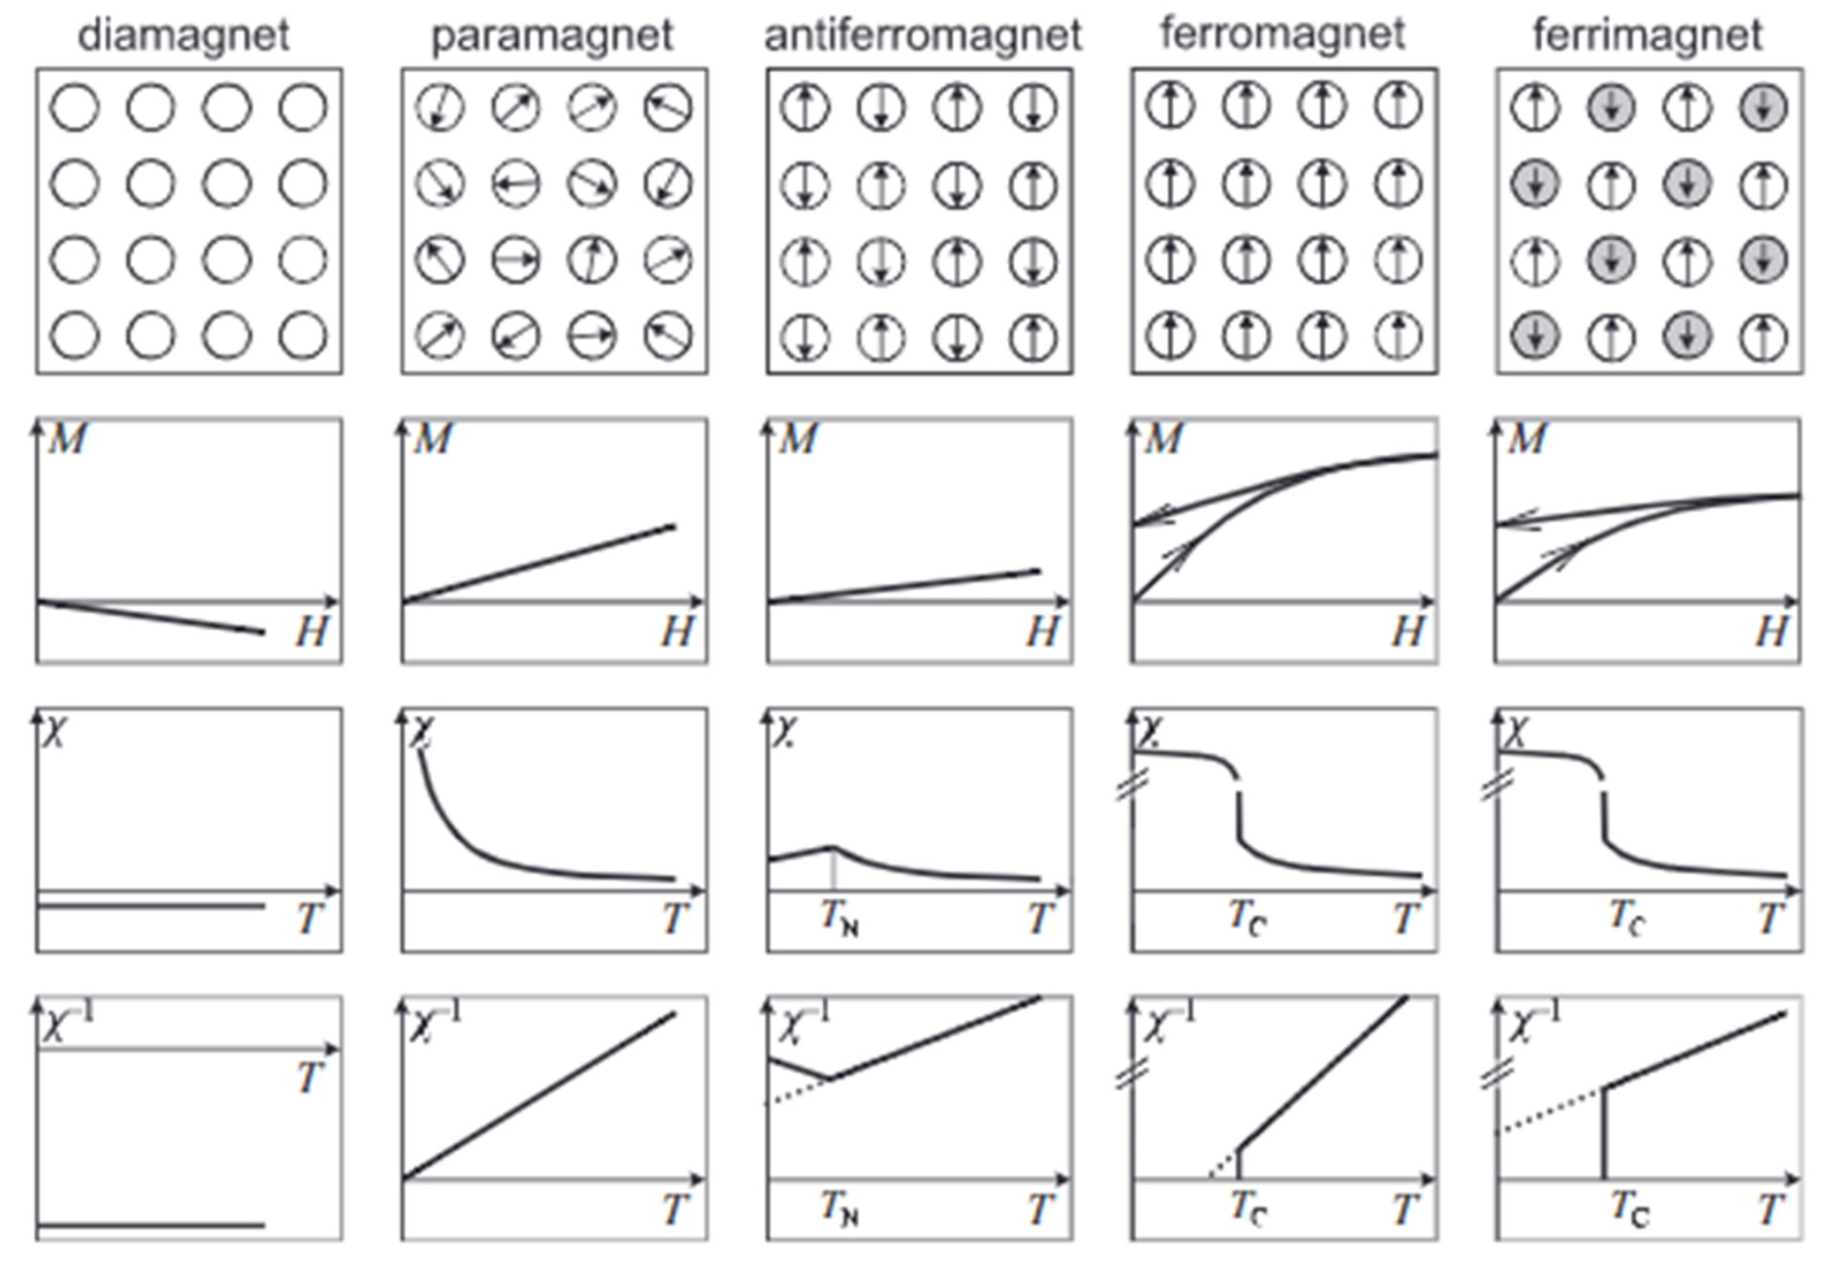
\includegraphics[width=0.65\linewidth]{bulkCoupling.png}
        \caption{Bulk magnetic coupling.}
        \label{fig:bulkCoupling}
    \end{table}
    \begin{itemize}
        \item Paramagnets have a bunch of spins with no preference for alignment. Note that $1/\chi$ is linear as discussed last lecture!
        \item Ferromagnet: We would need thermal energy to break the paired spins. This is an unstable equilibrium.
        \item Ferrimagnet: Closer to an antiferromagnet theoretically. Treats alloys where we have oppositely aligned differing spin populations. Behavior is almost exactly ferromagnetic.
    \end{itemize}
    \item Bulk behavior is dictated by nearest neighbor interactions.
    \begin{itemize}
        \item One exception is as follows, where the delocalized electron cloud can be polarized by a magnetic field.
    \end{itemize}
    \item \textbf{Pauli paramagnetism}: A metal that's a pool of electrons which are sloshing around in a band structure. Pool of positive and negative spins. Treat it as an electron gas. Applying a magnetic field changes the relative energies of the pool or electrons.
    \begin{figure}[h!]
        \centering
        \begin{tikzpicture}
            \begin{scope}
                \draw [blx,thick,name path=well]
                    (0,0) parabola (-1,1.8)
                    (0,-1) -- (0,2)
                    (0,0) parabola (1,1.8)
                ;
    
                \path [name path=int] (-1,1.3) -- ++(2,0);
                \begin{scope}[on background layer]
                    \fill [blz,name intersections={of=int and well}]
                        (0,0) parabola (intersection-1) -- (intersection-2) -- cycle
                        (0,0) parabola (intersection-3) -- (intersection-2) -- cycle
                    ;
                \end{scope}
                \node at (-0.48,1.6) {\Large$\upharpoonleft$};
                \node at (0.48,1.6) {\Large$\downharpoonright$};
            \end{scope}
            \draw [very thick,-latex] (1.5,0.5) -- node[above]{\footnotesize$B$} ++(2,0);
            \begin{scope}[xshift=5cm]
                \draw [blx,thick,name path=well]
                    (0,0) parabola (-1,1.8)
                    (0,-1) -- (0,2)
                    (0,-0.2) parabola (1,1.8)
                ;
    
                \path [name path=int] (-1,1.3) -- ++(2,0);
                \begin{scope}[on background layer]
                    \fill [blz,name intersections={of=int and well}]
                        (0,0) parabola (intersection-1) -- (intersection-2) -- cycle
                        (0,-0.2) parabola (intersection-3) -- (intersection-2) -- cycle
                    ;
                \end{scope}
                \node at (-0.48,1.6) {\Large$\upharpoonleft$};
                \node at (0.48,1.6) {\Large$\downharpoonright$};
            \end{scope}
        \end{tikzpicture}
        \caption{Pauli paramagnetism.}
        \label{fig:pauliParamag}
    \end{figure}
    \begin{itemize}
        \item We now have more spin down, creating a net magnetic field that will be very small. \emph{This} is Pauli paramagnetism.
    \end{itemize}
    \item Ferromagnets.
    \begin{itemize}
        \item Most applications for magnets are with ferromagnetic materials.
        \item \ce{NdFeB} is the strongest \textbf{hard} ferromagnet.
        \item The most classic case of a ferrimagnet is magnetite (mixed \ce{Fe^2+} and \ce{Fe^3+}).
    \end{itemize}
    \item Ferromagnets ideally have only one magnetic domain.
    \begin{figure}[h!]
        \centering
        \begin{tikzpicture}[
            every node/.style=black
        ]
            \begin{scope}
                \filldraw [draw=orx,fill=orz,thick] (-0.5,-0.7) rectangle node{\Large$\uparrow$} ++(1,1.4);
            \end{scope}
            \draw [very thick,-latex] (0.9,0) -- ++(1.2,0);
            \begin{scope}[xshift=3cm]
                \filldraw [draw=orx,fill=orz,thick] (-0.5,-0.7) rectangle node{\Large$\uparrow$} ++(0.5,1.4);
                \filldraw [draw=orx,fill=rez,thick] (0,-0.7) rectangle node{\Large$\downarrow$} ++(0.5,1.4);
            \end{scope}
            \draw [very thick,-latex] (3.9,0) -- ++(1.2,0);
            \begin{scope}[xshift=6cm]
                \filldraw [draw=orx,fill=orz,thick] (-0.5,-0.7) rectangle node{\Large$\uparrow$} ++(0.5,1.4);
                \filldraw [draw=orx,fill=rez,thick] (0,-0.7) rectangle node{\Large$\downarrow$} ++(0.5,1.4);
                \filldraw [draw=orx,fill=ylz,thick] (-0.5,-0.7) -- node[above=-1.5pt]{$\leftarrow$} ++(1,0) -- ++(-0.5,0.4) -- cycle;
                \filldraw [draw=orx,fill=ylt,thick] (-0.5,0.7) -- node[below=-1.5pt]{$\rightarrow$} ++(1,0) -- ++(-0.5,-0.4) -- cycle;
            \end{scope}
        \end{tikzpicture}
        \caption{Ferromagnetic domains.}
        \label{fig:FMdomains}
    \end{figure}
    \begin{itemize}
        \item Over time, different magnetic fields fracture domains. The products may align antiparallel.
        \item Applying a strong external magnetic field can anneal the domain walls and get you back to a single domain.
    \end{itemize}
    \item \textbf{Saturation magnetization}: The maximal magnetization of a material. \emph{Denoted by} $\bm{M_\textbf{sat}}$.
    \item \textbf{Remnant magnetization}: The magnetization of a magnetized material after the external field is dialed back. \emph{Denoted by} $\bm{M_\textbf{rem}}$.
    \item \textbf{Coercive field}: The amount of external field required to flip a magnet. \emph{Denoted by} $\bm{H_C}$.
    \item Visualizing $M_\text{sat}$, $M_\text{rem}$, and $H_C$.
    \begin{figure}[H]
        \centering
        \begin{tikzpicture}
            \small
            \draw
                (-2,0) -- (2,0) node[right]{$H$}
                (0,-2) -- (0,2) node[above]{$M$}
            ;
    
            \footnotesize
            \draw [rex,thick] (1.6,1.6) node[circle,fill,inner sep=1.5pt,label={above right:${\color{black}M_\text{sat}}$}]{}
                to[out=180,in=10,looseness=0.5] (0,1.5) node[circle,fill,inner sep=1.5pt,label={below right:${\color{black}M_\text{rem}}$}]{}
                to[out=-170,in=90] (-0.9,0) node[circle,fill,inner sep=1.5pt,label={below left:${\color{black}H_C}$}]{}
                to[out=-90,in=0] (-1.6,-1.6)
                to[out=0,in=-170,looseness=0.5] (0,-1.5)
                to[out=10,in=-90] (0.9,0)
                to[out=90,in=180] cycle
            ;
        \end{tikzpicture}
        \caption{Hysteresis loop.}
        \label{fig:hysteresis}
    \end{figure}
    \begin{itemize}
        \item A hysteresis loop characterizes the energy penalty to homogenize away domain boundaries and then flip the spin of a bulk domain; this quantity is what gives ferromagnets their useful properties.
        \item $H_C\propto\text{SOC}$, i.e., spin-orbit coupling.
        \item Things like \ce{Fe^3+} HS $d^5$ with equally (singly) occupied $d$ orbitals have no preferred orientation.
        \begin{itemize}
            \item \ce{Ti^3+} with $d^1$ can generate "ring currents," giving it a preferred orientation.
        \end{itemize}
        \item The wider the curve, the \textbf{harder} the ferromagnet.
        \item \textbf{Soft} is much skinnier (good for things like transformers that you want to be able to switch).
        \item To mediate coupling between $f$ orbitals in lanthanides, we mix in a bit of iron to use its free electrons.
    \end{itemize}
    \item Exotic things just to be aware of.
    \begin{itemize}
        \item Ferrometals: Iron is an example.
        \begin{itemize}
            \item Metallic band structure even in the absence of a magnetic field.
        \end{itemize}
        \item Ferro half metal.
        \begin{itemize}
            \item Charge carriers are spin-polarized.
            \item Important in spin-tronic type applications, P/N junctions, etc.
            \item Example: \ce{CrO2}.
        \end{itemize}
        \item Metals have a continuous set of bands at the Fermi level regardless.
        \item Ferro insulator.
        \begin{itemize}
            \item Filled band with no density of states. A magnet that is not conductive, essentially.
            \item Example: \ce{EuO}.
        \end{itemize}
        \item Weak coupling or frustration. AF exchange with spins that get frozen in. Frustration: Triangular lattice with up/down/what's the third.
        \item Spin glass: Freeze-in spin orientations such that when you get back to a certain magnetization, you auto-drop.
    \end{itemize}
    \item Magnetic properties of some anonymized commercial polycrystalline hard magnets.
    \item Do we have to learn the stuff at the end of the notes on exotic materials, ferrimagnetism, and commercial magnets??
    \item Next week: EPR.
\end{itemize}




\end{document}